\documentclass[a4paper]{article}

\usepackage{url}
\usepackage[T2A]{fontenc}
\usepackage[utf8]{inputenc}
\usepackage{graphicx}
\usepackage{wrapfig}
\usepackage[english,serbianc]{babel}

\usepackage[unicode]{hyperref}
\hypersetup{colorlinks=true,linkcolor=black,urlcolor=black,citecolor=black}

\usepackage{amsmath,amsthm,amssymb}
\usepackage{float}
\usepackage{xcolor}

\title{\textbf{Пеђа Стојаковић}}
\author{Ђорђе Славковић}
\date{\today}

\newtheorem{definicija}{Дефиниција}
\newtheorem{teorema}{Теорема}
\newtheorem{lema}{Лема}

\begin{document}

\maketitle

\newpage

\tableofcontents

\newpage

\section{Увод}

\textbf{Пеђа Стојаковић} је један од најпознатијих српских
кошаркаша и један од најбољих шутера своје генерације.
Рођен је 9. јуна 1977. године у Славонској Пожеги.

Кошарком је почео да се бави веома млад, а својим талентом
и великим бројем постигнутих поена брзо је привукао пажњу.
Током каријере наступао је у Европи и НБА лиги.

\section{Биографија}

\begin{wrapfigure}{r}{0.40\textwidth}
    \centering
    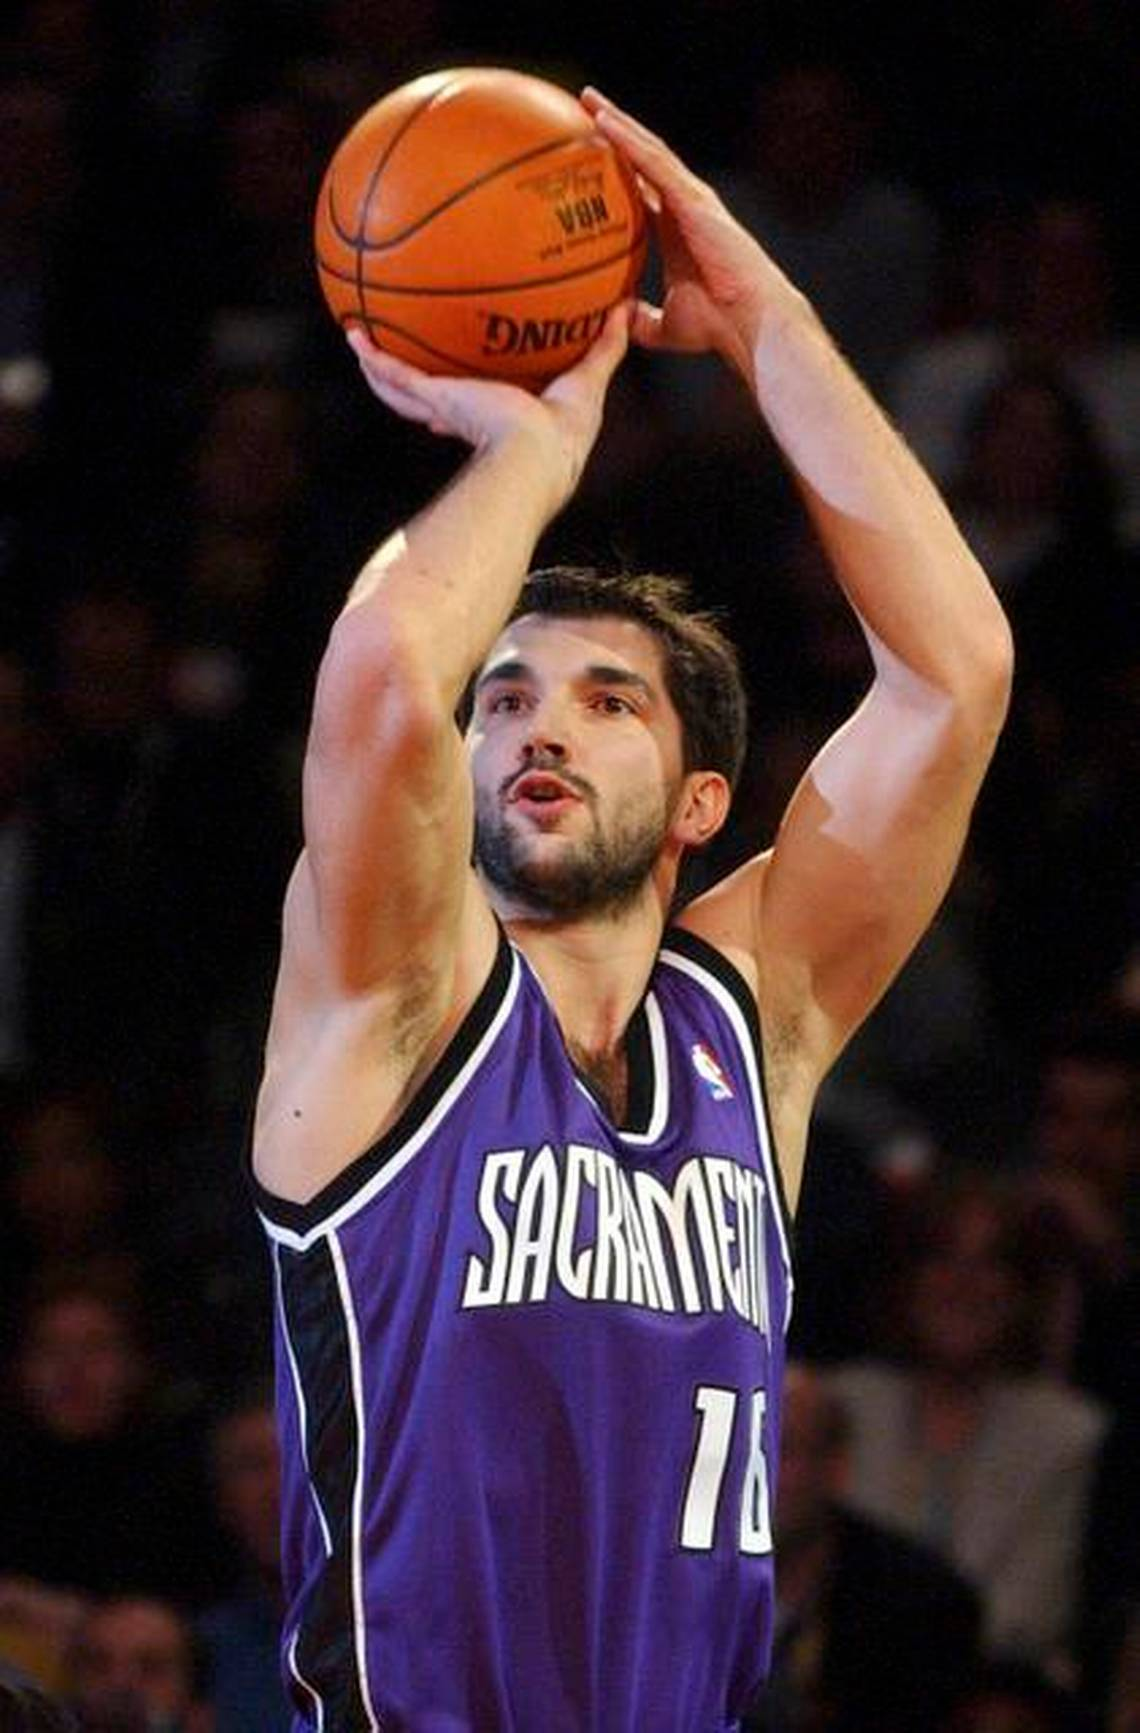
\includegraphics[width=0.37\textwidth]{slike/ps.jpg}
    \caption{Пеђа Стојаковић}
\end{wrapfigure}

Пеђа Стојаковић је бивши српски професионални кошаркаш.
Познат је по изузетно прецизном шуту за три поена и добрим
играчким способностима.

Током каријере постао је један од најпознатијих играча
Сакраменто Кингса. Његове игре у НБА лиги донеле су му
велику популарност широм света.

Његов стил игре карактерисали су \textit{прецизност},
добро кретање без лопте и одличан шут.

\subsection{Основни подаци}

\begin{table}[H]
\centering
\begin{tabular}{|c|c|}
\hline
\textbf{Податак} & \textbf{Информација} \\
\hline
Име и презиме & Пеђа Стојаковић \\
\hline
Датум рођења & 9. јун 1977. године \\
\hline
Место рођења & Славонска Пожега \\
\hline
Спорт & Кошарка \\
\hline
Позиција & Крилни играч \\
\hline
\end{tabular}
\caption{Основни подаци о Пеђи Стојаковићу}
\end{table}

\section{Каријера}

Пеђа Стојаковић је професионалну каријеру започео у Европи.
Наступао је за Црвену звезду и ПАОК, а затим је направио
велики корак преласком у НБА лигу.

Године 1996. изабран је на НБА драфту од стране
Сакраменто Кингса. У том клубу је постао један од
најважнијих играча и један од најбољих шутера лиге.

Током НБА каријере играо је и за:

\begin{itemize}
    \item Индијана Пејсерсе
    \item Њу Орлеанс Хорнетсе
    \item Торонто Репторсе
    \item Далас Мавериксе
\end{itemize}

Најзначајнији периоди његове каријере били су:

\begin{enumerate}
    \item Почетак професионалне каријере у Европи
    \item Прелазак у НБА лигу
    \item Успешни наступи за Сакраменто Кингсе
    \item Освајање НБА титуле са Далас Мавериксима
\end{enumerate}

\section{Трофеји и признања}

Пеђа Стојаковић је током своје каријере освојио
значајна екипна и индивидуална признања.

Посебно се издвајају златне медаље освојене са
репрезентацијом и НБА шампионска титула.

\begin{table}[H]
\centering
\begin{tabular}{|c|c|c|}
\hline
\textbf{Година} & \textbf{Такмичење} & \textbf{Успех} \\
\hline
2001. & Европско првенство & Златна медаља \\
\hline
2002. & Светско првенство & Златна медаља \\
\hline
2011. & НБА лига & НБА шампион \\
\hline
\end{tabular}
\caption{Најважнији успеси}
\end{table}

\subsection{Индивидуална признања}

Међу његовим значајним признањима издвајају се:

\begin{itemize}
    \item учешћа на НБА Ол-стар утакмицама,
    \item признања за једног од најбољих шутера,
    \item НБА шампионска титула,
    \item успеси са репрезентацијом.
\end{itemize}

\section{Математички пример}

Кошаркашка статистика се може представити математичким
формулама. На пример, проценат успешности шута може се
израчунати формулом:

\[
P = \frac{m}{n} \cdot 100\%
\]

где је $m$ број погодака, а $n$ укупан број покушаја.

Ако кошаркаш погоди 8 од 10 шутева, добијамо:

\[
P = \frac{8}{10} \cdot 100\% = 80\%
\]

Овакав начин израчунавања користи се за анализу успешности
играча током утакмица и целе сезоне.

\section{Дефиниција, лема и теорема}

\begin{definicija}
Проценат успешности шута представља однос броја успешно
реализованих шутева и укупног броја покушаја, помножен са 100.
\end{definicija}

\begin{lema}
Ако број постигнутих шутева расте, а број укупних покушаја
остаје исти, проценат успешности шута се повећава.
\end{lema}

\begin{teorema}
Проценат успешности кошаркаша не може бити већи од $100\%$,
јер број успешних шутева не може бити већи од укупног броја
покушаја.
\end{teorema}

\section{Закључак}

Пеђа Стојаковић је оставио велики траг у српској и светској
кошарци. Својим талентом, радом и прецизним шутем постао је
један од најпознатијих српских кошаркаша.

Посебно су значајни његови наступи за Сакраменто Кингсе,
успеси са репрезентацијом и освојена НБА титула.

\textcolor{blue}{Његова каријера представља пример да се
талентом, трудом и упорношћу могу постићи велики резултати.}

\end{document}

